\documentclass[spanish,xcolor=dvipsnames]{beamer}
\usetheme{Frankfurt}

\definecolor{links}{HTML}{2A1B81}
\hypersetup{colorlinks,linkcolor=,urlcolor=links}

\usepackage{hyperref}
\usepackage[utf8x]{inputenc}
\usepackage{makeidx}
\usepackage{color}
\makeindex

\hypersetup{
  pdftitle={Redis como Middleware Orientado a Mensajes (MoM)},
  pdfauthor={Maykel Moya},
  pdfproducer=PDFLaTeX,
}

\usepackage{fancyvrb}
\usepackage{color}

\makeatletter
\def\PY@reset{\let\PY@it=\relax \let\PY@bf=\relax%
    \let\PY@ul=\relax \let\PY@tc=\relax%
    \let\PY@bc=\relax \let\PY@ff=\relax}
\def\PY@tok#1{\csname PY@tok@#1\endcsname}
\def\PY@toks#1+{\ifx\relax#1\empty\else%
    \PY@tok{#1}\expandafter\PY@toks\fi}
\def\PY@do#1{\PY@bc{\PY@tc{\PY@ul{%
    \PY@it{\PY@bf{\PY@ff{#1}}}}}}}
\def\PY#1#2{\PY@reset\PY@toks#1+\relax+\PY@do{#2}}

\def\PY@tok@gd{\def\PY@tc##1{\textcolor[rgb]{0.63,0.00,0.00}{##1}}}
\def\PY@tok@gu{\let\PY@bf=\textbf\def\PY@tc##1{\textcolor[rgb]{0.50,0.00,0.50}{##1}}}
\def\PY@tok@gt{\def\PY@tc##1{\textcolor[rgb]{0.00,0.25,0.82}{##1}}}
\def\PY@tok@gs{\let\PY@bf=\textbf}
\def\PY@tok@gr{\def\PY@tc##1{\textcolor[rgb]{1.00,0.00,0.00}{##1}}}
\def\PY@tok@cm{\let\PY@it=\textit\def\PY@tc##1{\textcolor[rgb]{0.25,0.50,0.50}{##1}}}
\def\PY@tok@vg{\def\PY@tc##1{\textcolor[rgb]{0.10,0.09,0.49}{##1}}}
\def\PY@tok@m{\def\PY@tc##1{\textcolor[rgb]{0.40,0.40,0.40}{##1}}}
\def\PY@tok@mh{\def\PY@tc##1{\textcolor[rgb]{0.40,0.40,0.40}{##1}}}
\def\PY@tok@go{\def\PY@tc##1{\textcolor[rgb]{0.50,0.50,0.50}{##1}}}
\def\PY@tok@ge{\let\PY@it=\textit}
\def\PY@tok@vc{\def\PY@tc##1{\textcolor[rgb]{0.10,0.09,0.49}{##1}}}
\def\PY@tok@il{\def\PY@tc##1{\textcolor[rgb]{0.40,0.40,0.40}{##1}}}
\def\PY@tok@cs{\let\PY@it=\textit\def\PY@tc##1{\textcolor[rgb]{0.25,0.50,0.50}{##1}}}
\def\PY@tok@cp{\def\PY@tc##1{\textcolor[rgb]{0.74,0.48,0.00}{##1}}}
\def\PY@tok@gi{\def\PY@tc##1{\textcolor[rgb]{0.00,0.63,0.00}{##1}}}
\def\PY@tok@gh{\let\PY@bf=\textbf\def\PY@tc##1{\textcolor[rgb]{0.00,0.00,0.50}{##1}}}
\def\PY@tok@ni{\let\PY@bf=\textbf\def\PY@tc##1{\textcolor[rgb]{0.60,0.60,0.60}{##1}}}
\def\PY@tok@nl{\def\PY@tc##1{\textcolor[rgb]{0.63,0.63,0.00}{##1}}}
\def\PY@tok@nn{\let\PY@bf=\textbf\def\PY@tc##1{\textcolor[rgb]{0.00,0.00,1.00}{##1}}}
\def\PY@tok@no{\def\PY@tc##1{\textcolor[rgb]{0.53,0.00,0.00}{##1}}}
\def\PY@tok@na{\def\PY@tc##1{\textcolor[rgb]{0.49,0.56,0.16}{##1}}}
\def\PY@tok@nb{\def\PY@tc##1{\textcolor[rgb]{0.00,0.50,0.00}{##1}}}
\def\PY@tok@nc{\let\PY@bf=\textbf\def\PY@tc##1{\textcolor[rgb]{0.00,0.00,1.00}{##1}}}
\def\PY@tok@nd{\def\PY@tc##1{\textcolor[rgb]{0.67,0.13,1.00}{##1}}}
\def\PY@tok@ne{\let\PY@bf=\textbf\def\PY@tc##1{\textcolor[rgb]{0.82,0.25,0.23}{##1}}}
\def\PY@tok@nf{\def\PY@tc##1{\textcolor[rgb]{0.00,0.00,1.00}{##1}}}
\def\PY@tok@si{\let\PY@bf=\textbf\def\PY@tc##1{\textcolor[rgb]{0.73,0.40,0.53}{##1}}}
\def\PY@tok@s2{\def\PY@tc##1{\textcolor[rgb]{0.73,0.13,0.13}{##1}}}
\def\PY@tok@vi{\def\PY@tc##1{\textcolor[rgb]{0.10,0.09,0.49}{##1}}}
\def\PY@tok@nt{\let\PY@bf=\textbf\def\PY@tc##1{\textcolor[rgb]{0.00,0.50,0.00}{##1}}}
\def\PY@tok@nv{\def\PY@tc##1{\textcolor[rgb]{0.10,0.09,0.49}{##1}}}
\def\PY@tok@s1{\def\PY@tc##1{\textcolor[rgb]{0.73,0.13,0.13}{##1}}}
\def\PY@tok@sh{\def\PY@tc##1{\textcolor[rgb]{0.73,0.13,0.13}{##1}}}
\def\PY@tok@sc{\def\PY@tc##1{\textcolor[rgb]{0.73,0.13,0.13}{##1}}}
\def\PY@tok@sx{\def\PY@tc##1{\textcolor[rgb]{0.00,0.50,0.00}{##1}}}
\def\PY@tok@bp{\def\PY@tc##1{\textcolor[rgb]{0.00,0.50,0.00}{##1}}}
\def\PY@tok@c1{\let\PY@it=\textit\def\PY@tc##1{\textcolor[rgb]{0.25,0.50,0.50}{##1}}}
\def\PY@tok@kc{\let\PY@bf=\textbf\def\PY@tc##1{\textcolor[rgb]{0.00,0.50,0.00}{##1}}}
\def\PY@tok@c{\let\PY@it=\textit\def\PY@tc##1{\textcolor[rgb]{0.25,0.50,0.50}{##1}}}
\def\PY@tok@mf{\def\PY@tc##1{\textcolor[rgb]{0.40,0.40,0.40}{##1}}}
\def\PY@tok@err{\def\PY@bc##1{\fcolorbox[rgb]{1.00,0.00,0.00}{1,1,1}{##1}}}
\def\PY@tok@kd{\let\PY@bf=\textbf\def\PY@tc##1{\textcolor[rgb]{0.00,0.50,0.00}{##1}}}
\def\PY@tok@ss{\def\PY@tc##1{\textcolor[rgb]{0.10,0.09,0.49}{##1}}}
\def\PY@tok@sr{\def\PY@tc##1{\textcolor[rgb]{0.73,0.40,0.53}{##1}}}
\def\PY@tok@mo{\def\PY@tc##1{\textcolor[rgb]{0.40,0.40,0.40}{##1}}}
\def\PY@tok@kn{\let\PY@bf=\textbf\def\PY@tc##1{\textcolor[rgb]{0.00,0.50,0.00}{##1}}}
\def\PY@tok@mi{\def\PY@tc##1{\textcolor[rgb]{0.40,0.40,0.40}{##1}}}
\def\PY@tok@gp{\let\PY@bf=\textbf\def\PY@tc##1{\textcolor[rgb]{0.00,0.00,0.50}{##1}}}
\def\PY@tok@o{\def\PY@tc##1{\textcolor[rgb]{0.40,0.40,0.40}{##1}}}
\def\PY@tok@kr{\let\PY@bf=\textbf\def\PY@tc##1{\textcolor[rgb]{0.00,0.50,0.00}{##1}}}
\def\PY@tok@s{\def\PY@tc##1{\textcolor[rgb]{0.73,0.13,0.13}{##1}}}
\def\PY@tok@kp{\def\PY@tc##1{\textcolor[rgb]{0.00,0.50,0.00}{##1}}}
\def\PY@tok@w{\def\PY@tc##1{\textcolor[rgb]{0.73,0.73,0.73}{##1}}}
\def\PY@tok@kt{\def\PY@tc##1{\textcolor[rgb]{0.69,0.00,0.25}{##1}}}
\def\PY@tok@ow{\let\PY@bf=\textbf\def\PY@tc##1{\textcolor[rgb]{0.67,0.13,1.00}{##1}}}
\def\PY@tok@sb{\def\PY@tc##1{\textcolor[rgb]{0.73,0.13,0.13}{##1}}}
\def\PY@tok@k{\let\PY@bf=\textbf\def\PY@tc##1{\textcolor[rgb]{0.00,0.50,0.00}{##1}}}
\def\PY@tok@se{\let\PY@bf=\textbf\def\PY@tc##1{\textcolor[rgb]{0.73,0.40,0.13}{##1}}}
\def\PY@tok@sd{\let\PY@it=\textit\def\PY@tc##1{\textcolor[rgb]{0.73,0.13,0.13}{##1}}}

\def\PYZbs{\char`\\}
\def\PYZus{\char`\_}
\def\PYZob{\char`\{}
\def\PYZcb{\char`\}}
\def\PYZca{\char`\^}
\def\PYZsh{\char`\#}
\def\PYZpc{\char`\%}
\def\PYZdl{\char`\$}
\def\PYZti{\char`\~}
% for compatibility with earlier versions
\def\PYZat{@}
\def\PYZlb{[}
\def\PYZrb{]}
\makeatother


\beamertemplatenavigationsymbolsempty

\title{Redis como \textit{Middleware} Orientado a Mensajes (MoM)}
\author[Maykel Moya]{Maykel Moya}
\institute[URJC]{
  Máster en Sistemas Telemáticos e Informáticos \\
  Universidad Rey Juan Carlos \\
  Madrid
}
\date{abril 2012}

\begin{document}

\begin{frame}[plain]
  \titlepage
\end{frame}

\begin{frame}[plain]
  \vspace{6cm}
  \tiny
  \hfill \copyright 2012 Maykel Moya \\
  \hfill Algunos derechos reservados \\
  \hfill Este trabajo se distribuye bajo la licencia \\
  \hfill 
\includegraphics[width=15mm]{images/by-nc-sa.png} \\
  \hfill Creative Commons Attribución-NoComercial-CompartirIgual \\
  \hfill disponible en \url{http://creativecommons.org/licenses/by-nc-sa/3.0/deed.es} \\
\end{frame}

\begin{frame}[plain]{Agenda}
  \tableofcontents[]
\end{frame}

\section{Memcached}

\begin{frame}{En el principio fue Memcached}
  \begin{itemize}\addtolength{\itemsep}{0.5\baselineskip}
    \item Servidor de caché (acceso por la red)
    \item Sólo comandos \texttt{GET} y \texttt{SET} (simple)
    \item Alto rendimiento
    \item Almacenamiento en memoria (volátil)
    \item Almacenamiento basado en llave/valor
    \item Software Libre
    \item \url{http://memcached.org/}
  \end{itemize}
\end{frame}

\begin{frame}{Uso típico}
  Sólo comandos \texttt{GET} y \texttt{SET}
  \begin{columns}
    \begin{column}{0.50\textwidth}
      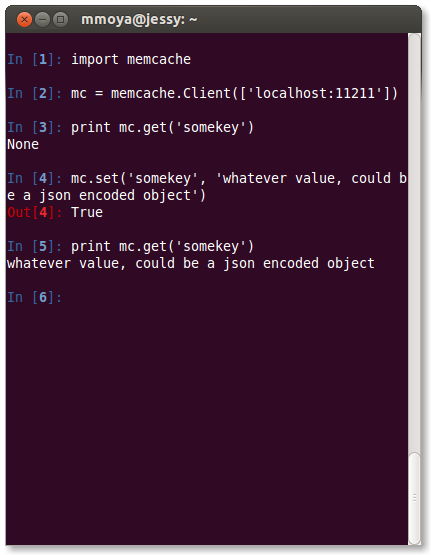
\includegraphics[width=\linewidth]{images/memcache-interactive-session.png}
    \end{column}
    \pause
    \begin{column}{0.40\textwidth}
      \tiny
      \include{memcache-example}
    \end{column}
  \end{columns}
\end{frame}

\section{Redis}

\begin{frame}{Luego Redis}
  \begin{itemize}\addtolength{\itemsep}{0.5\baselineskip}
    \item Servidor de caché (acceso por la red)
    \item Alto rendimiento
    \item Almacenamiento persistente
    \item Almacenamiento basado en llave/valor
    \begin{itemize}
      \item Pero los valores pueden ser \textit{strings},
        \textit{hashes}, \textit{lists} entre otros
      \item ... por lo que se conoce también como Servidor de
        Estructuras de Datos
    \end{itemize}
    \item Software Libre
    \item \url{http://redis.io/}
  \end{itemize}
\end{frame}

\begin{frame}{Comandos}
  \begin{itemize}
    \item Además de los básicos \texttt{GET} y \texttt{SET}
  \end{itemize}
  \begin{itemize}
    \item \texttt{LPUSH}: Inserción de un elemento al principio de una lista (\textit{Left PUSH})
    \item \texttt{RPOP}: Eliminación de un elemento del final de una lista (\textit{Right POP})
    \item \texttt{BRPOP}: Idem pero bloqueante (\textit{Blocking Right POP})
    \item \texttt{PUBLISH}: Publicación en un canal
    \item \texttt{SUBSCRIBE}: Subscripción a un canal
    \item \texttt{UNSUBSCRIBE}: Cancelar subscripción a un canal
    \item \textit{muchos otros}
  \end{itemize}
  \begin{itemize}
    \item \url{http://redis.io/commands}
  \end{itemize}
\end{frame}

\section{Redis como MoM}

\begin{frame}{\textit{Middleware} Orientado a Mensajes (MoM)}
% https://en.wikipedia.org/wiki/Message-oriented_middleware
  \begin{block}{De Wikipedia:}
    \begin{quotation}
       ... infraestructura de software o hardware que permite el envío
       y recepción de mensajes entre componentes de un sistema
       distribuido
     \end{quotation}
  \end{block}
\end{frame}

\begin{frame}{Paradigmas de distribución en un MoM}
  \begin{center}
  \begin{tabular}{ l || p{2cm} | p{2cm} | p{2cm} }
                 & \scriptsize cuántos suscriptores reciben el mensaje?
                 & \scriptsize se retiene el mensaje?
                 & \scriptsize se puede implementar con Redis? \\
    \hline\hline
    \textit{queue}                & uno   & sí & sí \\
    \textit{topic}                & todos & no & sí \\
    \textit{durable subscription} & todos & sí & sí \\
  \end{tabular}
  \end{center}

  \pause

  \vspace{\baselineskip}

  ¿Cómo se implementa con Redis?

  \begin{itemize}\addtolength{\itemsep}{0.5\baselineskip}
    \item \textit{Queue}: Con \texttt{LPUSH} y \texttt{BRPOP}
    \pause
    \item \textit{Topic}: Con \texttt{SUBSCRIBE} y \texttt{PUBLISH}
    \pause
    \item \textit{Durable Subscription}: Con \texttt{SUBSCRIBE}, \texttt{PUBLISH}
      y \textit{Sorted Sets}, ver \url{http://j.mp/JBjwdT}.
  \end{itemize}
\end{frame}

\section{Demo}

\begin{frame}
  \begin{center}
  \Huge
  Y ahora el demo!
  \end{center}
\end{frame}

\begin{frame}[plain]{Preguntas}
   
\includegraphics[width=\linewidth]{images/question.png}
\end{frame}

\begin{frame}[plain]{Referencias}
  \begin{enumerate}\addtolength{\itemsep}{0.5\baselineskip}
    \item \href{http://www.darkcoding.net/software/choosing-a-message-queue-for-python-on-ubuntu-on-a-vps/}
               {Choosing a message queue for Python on Ubuntu on a VPS}.
    \item \href{http://stackoverflow.com/questions/7871526/is-non-blocking-redis-pubsub-possible}
               {Is non-blocking Redis pubsub possible?}.
    \item \href{http://redis.io/topics/pubsub}
               {Redis Pub/Sub}.
    \item \href{http://stackoverflow.com/a/7672670/253049}
               {Does the redis pub/sub model require persistent connections to redis?}.
    \item \href{http://pkghosh.wordpress.com/2012/03/28/redis-as-messaging-middleware/}
               {Redis as Messaging Middleware}.
    \item \href{http://blog.joshsoftware.com/2011/01/03/do-you-need-a-push-notification-manager-redis-pubsub-to-the-rescue/}
               {Do you need a Push Notification Manager? – Redis PubSub to the rescue}.
  \end{enumerate}
\end{frame}

\end{document}
